\begin{surferPage}[Singularitat A4++]{Una singularitat $A_4^{++}$}
Com ja s'ha vist, una $A_4^{+-}$ s'assembla a una $A_2^{+-}$.
Anàlogament,
$A_4^{++}$ i $A_2^{++}$ són quasi idèntiques.
Les imatges següents mostren superfícies
    $A_2^{++}$, $A_4^{++}$,$A_2^{+-}$, $A_4^{+-}$:
    \begin{center}
      \vspace*{-0.2cm}
      \begin{tabular}{@{}c@{\ }c@{\ }c@{\ }c@{}}
        \begin{tabular}{@{}c@{}}
          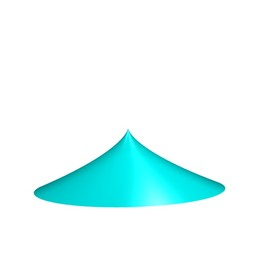
\includegraphics[width=1.2cm]{../../common/images/A2pp}
        \end{tabular}
        &
        \begin{tabular}{@{}c@{}}
          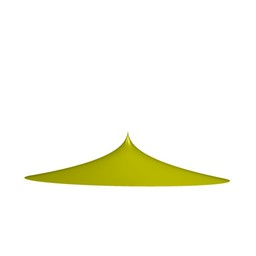
\includegraphics[width=1.2cm]{../../common/images/A4pp}
        \end{tabular}
        &
        \begin{tabular}{@{}c@{}}
          
\includegraphics[width=1.2cm]{../../common/images/A2pm}
        \end{tabular}
        &
        \begin{tabular}{@{}c@{}}
          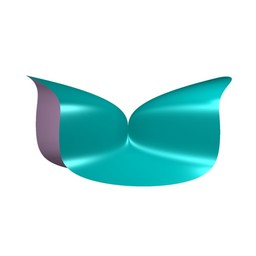
\includegraphics[width=1.2cm]{../../common/images/A4pm}
        \end{tabular}
      \end{tabular}
    \end{center}
    \vspace*{-0.2cm}
S'observa que les superfícies
$A_4$ s'apropen al punt singular més sobtadament que les $A_2$.

Com en el cas de la $A_4^{+-}$, s'obté una diferència crucial
amb la $A_2$ només quan intentem deformar la singularitat en
singularitats  còniques o en una superfície amb diversos forats: la
singularitat $A_2^{++}$ només es pot deformar en una singularitat
cònica. Mentre que $A_4^{++}$ ho fa en dues:
%    \dontshow{
    %
    \begin{center}
      \vspace*{-0.2cm}
      \begin{tabular}{@{}c@{\quad}c@{\quad}c@{}}
        \begin{tabular}{@{}c@{}}
          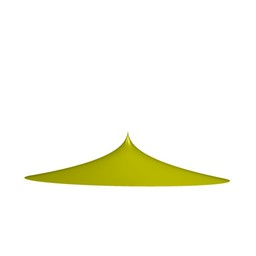
\includegraphics[width=1.2cm]{../../common/images/A4pp_0}
        \end{tabular}
        &
        \begin{tabular}{@{}c@{}}
          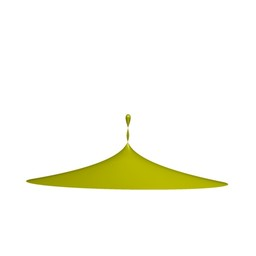
\includegraphics[width=1.2cm]{../../common/images/A4pp_1}
        \end{tabular}
        &
        \begin{tabular}{@{}c@{}}
          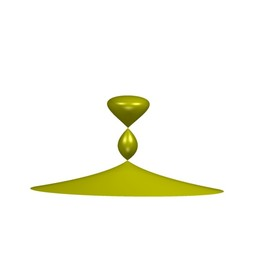
\includegraphics[width=1.2cm]{../../common/images/A4pp_2}
        \end{tabular}
      \end{tabular}
    \end{center}
%    }
      \vspace*{-0.2cm}
Això s'aconsegueix amb l'equació
    \[x^2(x+a^2)^2(x-a^2)+y^2+z^2.\]
 
\end{surferPage}
